\chapter{Network Measurements}
\label{chp:measurements2}


This chapter will display the experiments conducted on data sending rate from the nRF52 to the Raspberry Pi in the form of and graphs, tables and figures to try to determine the most efficient combination of amount of data to send, sending frequency as well as protocols to use. 

%\section{temp/notes}

%Trying to understand the details of a capture in Wireshark. 

%Can fragmentation give us an advangate, if you can send more data pr header. 

%An empty char array sent over CoAP is 76 bytes. 
%19 bytes char array, 96 bytes
%21 bytes char array, 98 bytes. Adds only as much as needed. 
 

\section{Initial limitations in the Network}

\subsection{Stable transfer rate}

As soon as the end nodes of the network can communicate with the Raspberry Pi, the next step is to test the transfer rate of the connection. To measure the network transfer rate, \textit{ping6} was used. This is a software tool used to test networks using \gls{ipv6} in a network. The results is measured in ms used for every \gls{rtt}. 

\begin{verbatim}
ping6 2001::2e6:6aff:fe64:54dd
ping6 google.com
\end{verbatim}

\begin{figure}[ht]
    \centering
    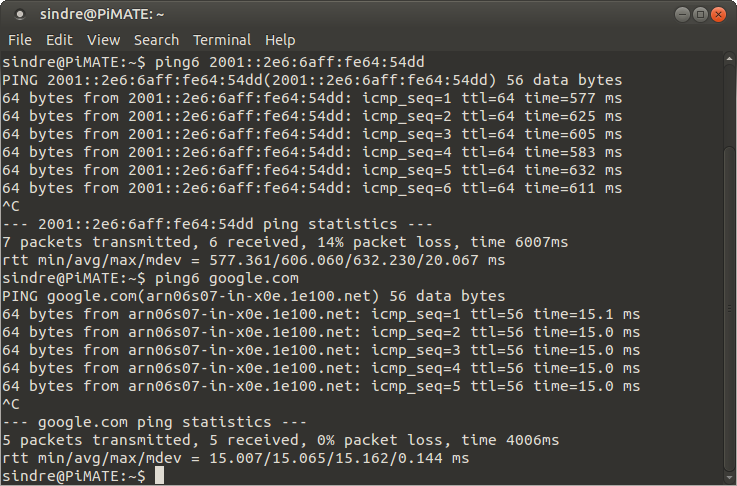
\includegraphics[scale=0.5]{ping6test.png}    
    \caption{Comparison: ping nRF52 and ping google.com}
    \label{fig:pingComparison}
\end{figure}

When tested, the connection turns out to be very slow and in some cases very unstable, especially at maximum transfer rate. In the test of ping shown in figure \ref{fig:pingComparison} the connection between the Raspberry Pi and the nRF52 had 14 \% packet loss, 1 out of 7 packets. Other test showed similar results, but the \gls{coap} \gls{con} has in general got a  higher stability at maximum sending rate than \gls{coap} \gls{non}. After a test period it was therefore decided that the best solution for \gls{non} would be to gather data from sensors at a higher rate, and store them in the nRF52 temporarily. Every second all the measured values are being transferred to the Raspberry Pi, the temporarily values are deleted and the measurement continues. This has proven to be a very stable solution, with successful tests over several days. \gls{con} can handle more frequent transportations than this in this system, on average 4 times per second. See the test shown in chapter \ref{chp:measurements2}.6. \todo{Make figure}. 

\begin{equation} \label{avg_eq}
    \overline{x}_{n} = \frac{\sum\limits_{i=1}^n x_{i}}{n}
\end{equation}

Equation \ref{avg_eq} shows the standard way used to calculate an average of the measured values. Here \textit{a} is any real number and \textit{n} is any integer. 

After a test period, the problems explained in \todo {Skriv om problemer med bt8 i Architecture?} was fixed. A more reliable test could then be performed, as shown in figure \ref{fig:ping2}. Using equation \ref{avg_eq} to calculate average gives an approximate average of 250 ms \gls{rtt}. This is very slow, and way beneath the transfer limitations of both \gls{ble}, \gls{6lowpan} and \gls{coap}, as explained in chapter \ref{chp:background} \todo{Skriv spesifikt om begrensninger for disse tre i background}. Another factor could be limited power supply and computational power, but it is not clear what is the main cause at this point. This will regardless be a huge limitation in the network. 

\begin{figure}[ht]
    \centering
    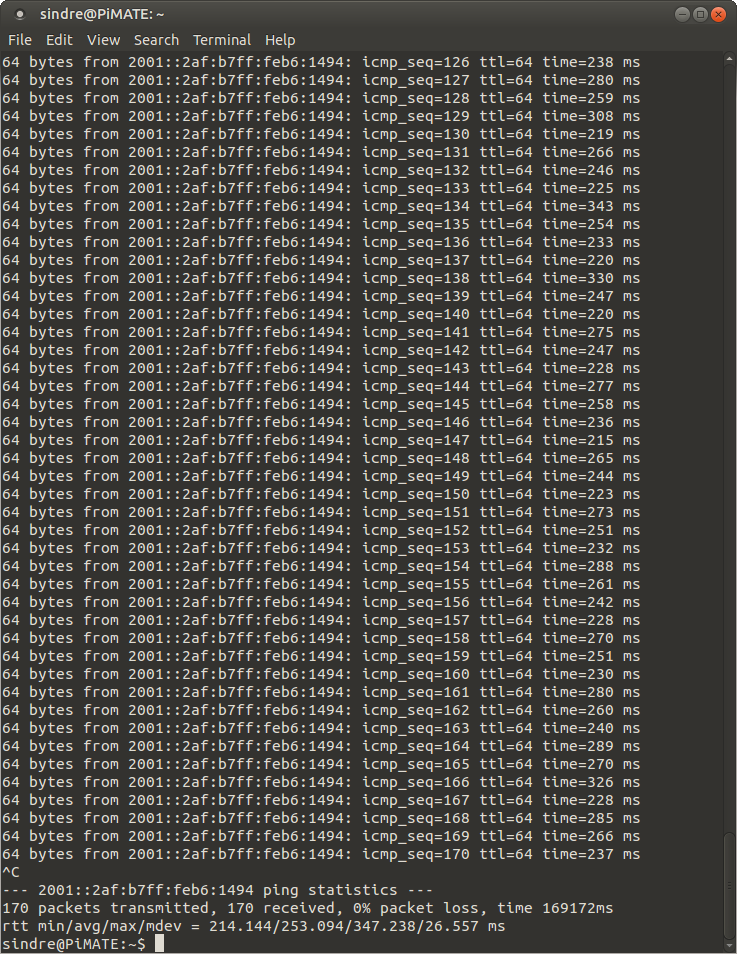
\includegraphics[scale=0.4]{ping3.png}    
    \caption{Ping nRF52, different time}
    \label{fig:ping2}
\end{figure}


The conclusion from these initial tests is therefore that \gls{coap} \gls{con} is stable at at lower transfer interval than \gls{coap} \gls{non}, and can in best case cope with sending every 250th ms, which is very good compared to the high \gls{rtt}. \gls{non} has been so unstable at initial tests that it was decided to only send every second. This makes quite a huge difference when testing the different protocols, as \textit{CoAP CON} can send a lot more \textit{goodput} per second, but \textit{CoAP NON} requires less power to send each message, and a much higher percentage of the packets sent through the network contains useful data.


\subsection{Packet fragmentation}

In Internet Routing, \textit{fragmentation} is known as the action of splitting data into smaller packets, to satisfy the maximal limits of the different technologies or protocols used (e.g. \gls{ble} and \gls{6lowpan} in the network described in this thesis). Each of these packets needs header fields of a certain size, or other requirements. In a network of microcontrollers used in this thesis fragmentation can be a factor that needs to be taken into account to optimize the goodput of the system. This will be a central part of the testing, and will therefore be explained in detail in the following section. 

To better understand fragmentation, imagine a train with carriages as shown in Figure \ref{fig:trainExample}. To be able to operate at all, the train needs a locomotive with an engine driver, a conductor and a cafe carriage. As soon as these things are already there, the company owning the train gets better and better off for every passenger buying a ticket. Lets assume that every carriage can carry 4 employees and 27 passengers, to make it directly comparable to the \gls{ble} packets in the network. Eventually all the carriages will be full, and a decision has to be made if it will be profitable to fit another carriage. It will in general be most profitable to use as many carriages as the locomotive can handle, and to fill up every carriage as much as possible. It will however not be a good idea to connect another carriage if there will only be one additional passenger sitting there, since the extra weight of the carriage adds unnecessary additional weight to the train set compared to the income. 

\begin{figure}[ht]
    \centering
    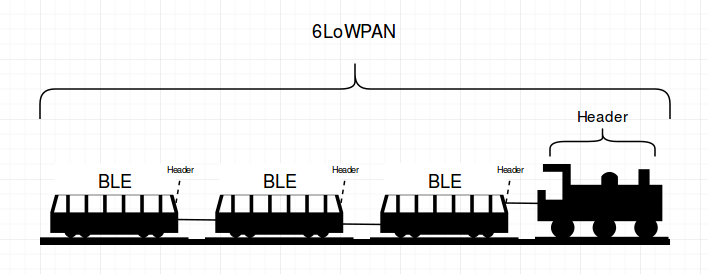
\includegraphics[scale=0.5]{trainExample.png}    
    \caption{Packet fragmentation - train comparison}
    \label{fig:trainExample}
\end{figure}

In this example, the locomotive and employees are the \gls{6lowpan} packet, that are needed no matter what to get the train working. Each additional carriage is a \gls{ble} packet. The goal is therefore to find the maximal number of passengers compared to the cost of adding additional carriages, in other words the maximal number of bytes compared to the number of packets sent. This is known as \textit{fragmentation}, fragmenting data into smaller pieces to satisfy the maximal limitations of packet sizes in the different protocols. This can be exploited by a system developer to maximize \textit{goodput} vs \textit{throughput} in the network.
 


\section{Description of measurements}

The following sections will show experiments performed to to test if \textit{fragmentation} is a huge issiue when sending data through low energy networks, and which of the protocols described in chapter \ref{chp:background}  is the most efficient to use when the goal is to get as high \textit{googput} as possible. This will be done by sending data of constant length, capture packets using \textit{Wireshark}, and then increasing the packet size to see the changes. 

Before these experiements started, the expected results was that sending a small amount of data at a time would not be preferable, because of the needed bytes to set up the connection, header files and so on. It was not known how big the packages needed to be before it would be considered \textit{profitable} to send. 

When sending \gls{ble} packets over the network, observations from the system shows that the maximum packet size over \gls{ble} is 31 bytes. Each of these packages needs a header field of 4 bytes, meaning 27 bytes left for useful data. However, to start the connection at all, 76 byte is needed, meaning three \gls{ble} packets. The ratio between \textit{useful} and \textit{needed} (known as \textit{goodput} and \textit{throughput}) data transferred therefore start out very poorly if the payload sent is very small.The best possible percentage of useful data we can hope to acheive will also be limited by this, 27 bytes goodput and 4 bytes header field, shown in the following calculation.  

\begin{equation} \label{percentage_eq} 
	\delta = \frac{x_{2}}{x_{1}} * 100 \%
\end{equation}

Equation \ref{percentage_eq} shows the standard way used to calculate the percentage, \textdelta , that the natural number \textit{x\textsubscript{2}} is of the total amount \textit{x\textsubscript{1}}. 

\begin{equation}
    \frac{27 b}{31 b}*100 \% = 87,094776 \% \approx 87,1 \%
\end{equation}





In the actual system the number will quite certain be a lot lower than this. Both because header files in \gls{6lowpan} packages needs to use some of the capacity, and because of other limitations\todo{Like what?}. 


\section{CoAP}

As explained in Chapter \ref{chp:measurements2}.1.1, \gls{coap} can be split into two different main sections. \gls{con} messages can be sent quite frequently, but every message needs to get an \gls{ack} before the next message can be sent. This means that it is quite fast, but a lot of packets needs to be transported through to get usable data at the other end. The other alternative is \gls{non}, where each message does \textit{not} need an \gls{ack}. 


%\begin{figure}[ht]
%    \centering
%    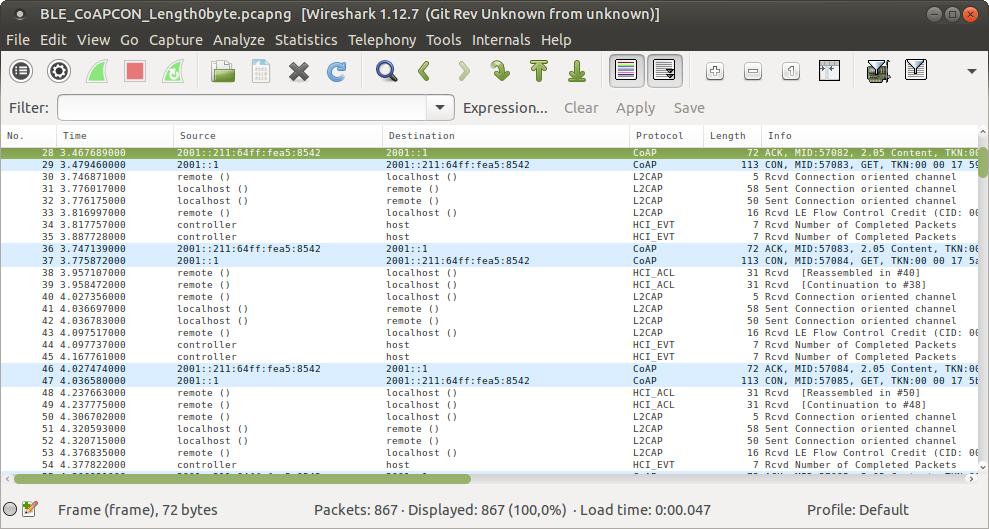
\includegraphics[width=\textwidth]{wiresharkCoAPCON0byte.png}    
%    \caption{Wireshark capture, CoAP CON, 0 bytes goodput}
%    \label{fig:coapCON0Wireshark}
%\end{figure}



%\begin{figure}[ht]
%    \centering
%    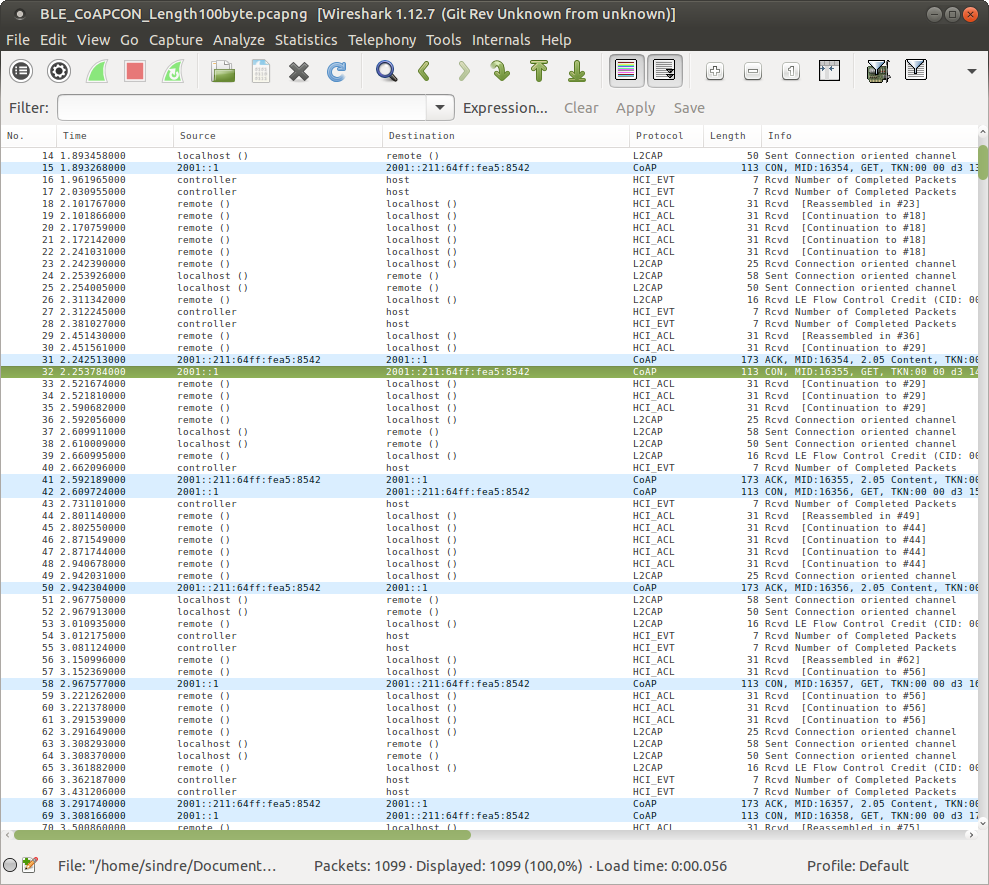
\includegraphics[width=\textwidth]{wiresharkCON100bytes.png}    
%    \caption{Wireshark capture, CoAP CON, 100 bytes goodput}
%    \label{fig:coapCON100Wireshark}
%\end{figure}

\begin{table}[ht]
\centering
\caption{Wireshark CoAP CON 0 bytes}
\label{coapCON0table}
\begin{tabular}{lllll}
Number & Time   & Protocol & Length & Info                             \\ \hline
36     & 3.7471 & CoAP     & 72     & ACK, MID:57083, 2.05 Content     \\
37     & 3.7759 & CoAP     & 113    & CON, MID:57084, GET              \\
38     & 3.9571 & HCI\_ACL & 31     & Rcvd {[}Reassembled in \#40{]}   \\
39     & 3.9584 & HCI\_ACL & 31     & Rcvd {[}Continuation to \#38{]}  \\
40     & 4.0274 & L2CAP    & 5      & Rcvd Connection oriented channel \\
41     & 4.0367 & L2CAP    & 58     & Sent Connection oriented channel \\
42     & 4.0368 & L2CAP    & 50     & Sent Connection oriented channel \\
43     & 4.0975 & L2CAP    & 16     & Rcvd LE Flow Control             \\
44     & 4.0977 & HCI\_EVT & 7      & Rcvd Number of Completed Packets \\
45     & 4.1678 & HCI\_EVT & 7      & Rcvd Number of Completed Packets \\
46     & 4.0275 & CoAP     & 72     & ACK, MID:57084, 2.05 Content     \\
47     & 4.0366 & CoAP     & 113    & CON, MID:57085, GET              \\ \hline
\end{tabular}
\end{table}

Table \ref{coapCON0table} shows the most basic example of a capture of packets in Wireshark \footnote{When measuring packet sizes, all measurements had the same result when the size of data was constant. The tables therefore takes only one of the measurements at a time in account. All the measured data can be found on \url{https://www.github.com/sische/MasterThesis}}. The full capture can be seen in the Appendix \ref{chp:appendix}. In this case an empty char array was sent, meaning an goodput equal to 0 byte. All of these bytes are therefore sent to route packages through the network. The maximum of 31 bytes per \gls{ble} packet have been exceeded twice, meaning that three packets needed to be sent. The first packet is labeled \textit{[Reassembled in \#40]}, the second \textit{[Continuation to \#38]} and the last \textit{Connection oriented channel}. After this, the \gls{ack} packages follows, two packages of 58 and 50 bytes, respectively. The last bytes received tells how many packages was completed, as a built in feature in \gls{ble}  \gls{hci}  and \gls{acl}. All of these packages can fit into one \gls{6lowpan} packet, since the total number of bytes are less than 270 bytes. 

Note that packet number 46 and 47 in table \ref{coapCON0table} has got a timestamp that indicates that they originally was sent from the end node in the network as packet number 41 and 42, but used longer time than the other packets sent through the network at the same time. The main reason for this is of course that they are bigger than the rest of the packets, but since the network limit should be much higher than this it can maybe be seen as a weakness that this gives a clear impact even at these small values.  


\begin{table}[]
\centering
\caption{Wireshark CoAP CON 100 bytes}
\label{coapCON100table}
\begin{tabular}{lllll}
Number & Time   & Protocol & Length & Info                             \\ \hline
29     & 2.4514 & HCI\_ACL & 31     & Rcvd {[}Reassembled in \#36{]}   \\
30     & 2.4516 & HCI\_ACL & 31     & Rcvd {[}Continuation to \#29{]}  \\
31     & 2.2425 & CoAP     & 173    & ACK, MID:16354, 2.05 Content     \\
32     & 2.2538 & CoAP     & 113    & CON, MID:16355, GET              \\
33     & 2.5217 & HCI\_ACL & 31     & Rcvd {[}Continuation to \#29{]}  \\
34     & 2.5218 & HCI\_ACL & 31     & Rcvd {[}Continuation to \#29{]}  \\
35     & 2.5907 & HCI\_ACL & 31     & Rcvd {[}Continuation to \#29{]}  \\
36     & 2.5921 & L2CAP    & 25     & Rcvd Connection oriented channel \\
37     & 2.6099 & L2CAP    & 58     & Sent Connection oriented channel \\
38     & 2.6100 & L2CAP    & 50     & Sent Connection oriented channel \\
39     & 2.6610 & L2CAP    & 16     & Rcvd LE Flow Control             \\
40     & 2.6621 & HCI\_EVT & 7      & Rcvd Number of Completed Packets \\
41     & 2.5922 & CoAP     & 173    & ACK, MID:16355, 2.05 Content     \\
42     & 2.3097 & CoAP     & 113    & CON, MID:16356, GET              \\ 
43     & 2.7311 & HCI\_EVT & 7      & Rcvd Number of Completed Packets \\ \hline
\end{tabular}
\end{table}

In table \ref{coapCON100table}, 100 bytes of goodput is being sent through. The same basic packages needed are still there, but in addition the 100 bytes of data is added. This means adding more \gls{ble} packets, but also that the percentage of useful data sent through is a lot higher, approximatley 55 \% in this case. By doing several experiments like this, it was possible to create the graph in Figure \ref{fig:coapCON0200}. This shows the correlation between goodput and throughput compared to the number of packets sent, measured every 10th byte from 0 byte to 200 bytes large packets.


\begin{figure}[ht]
    \centering
    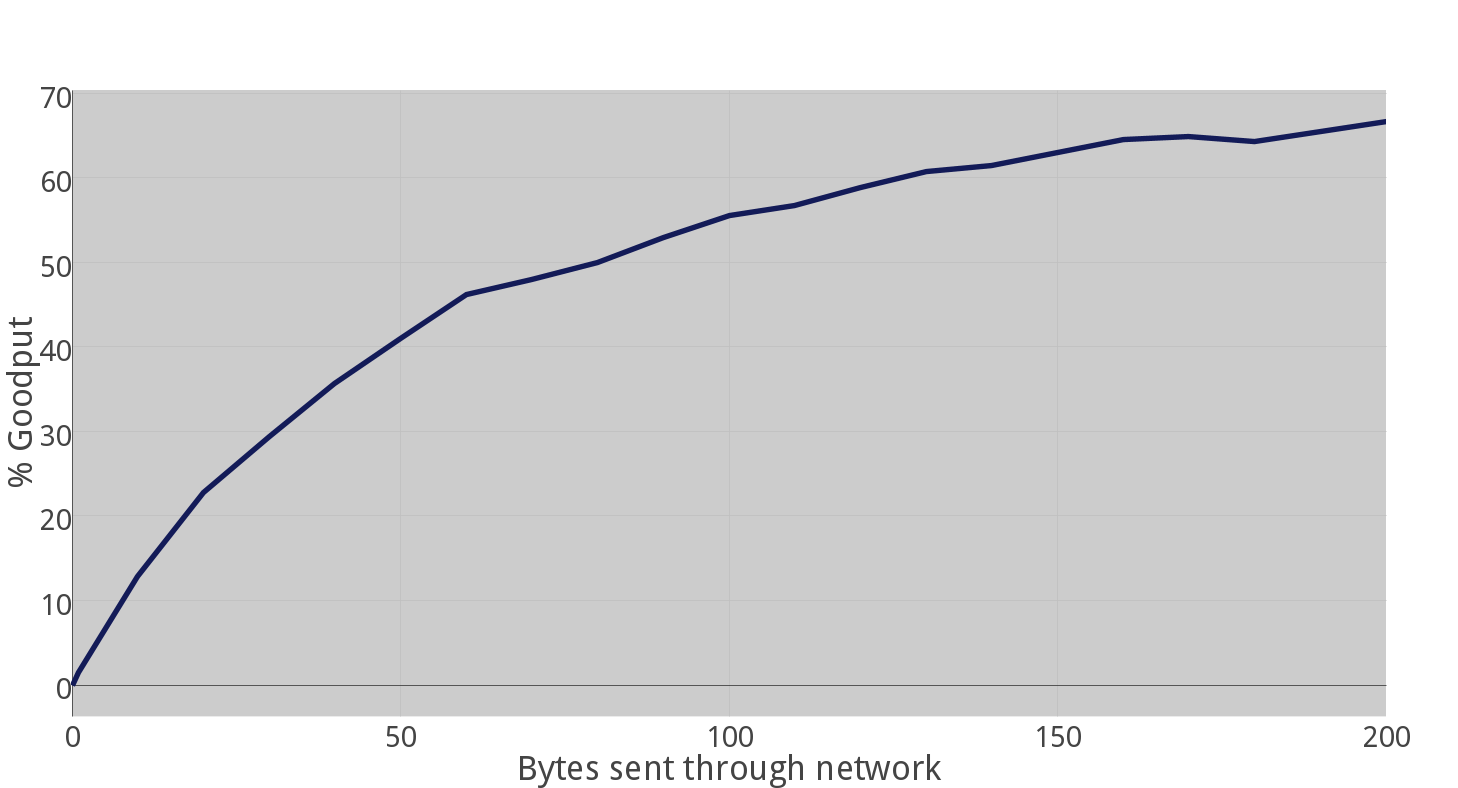
\includegraphics[scale=1.0]{CON0to200plot09thickerGRAY.png}    
    \caption{CoAP CON, 0-200 bytes sent}
    \label{fig:coapCON0200}
\end{figure}



In this particular case shown in \ref{fig:coapCON0200} it makes no sense to send less than 50 bytes of useful data at once, since more than 50 \% of the bytes sent will be header files. This is comparable to having a locomotive and full crew at disposal, but only a few or none paying passengers. The best possible result is to have every carriage full, with 27 passengers and 4 employees. Since at least 4 bytes out of every 31 sent needs to be used to header information, the best possible result will be 87,1 \%, as shown in equation 4.1. In mathematics, this is described as a \textit{horizontal asymptote} since the distance between the graph and \textit{y = 87,1} will approach zero after an infinite number of bytes has been transferred. The graph will therefore converge to 87,1 \%, just as the values climbing in figure \ref{fig:coapCON0200}, even before packet size of 200 bytes.  

\subsection{Discussion}

Even though this first test was done with a very limited amount of data transferred, it is easy to see that the curve clearly flattens out and forms the shape of a \textit{\gls{parabola}} with a vertical \textit{\gls{directrix}} at \textit{x = 0}. The next step would be to transfer a larger amount of data, to verify that the assumptions that the graph will converge to the asymptotic value \textit{y = 87,1} when $lim_{x\to\infty}$. The limitations of transfer rate is not nearly yet met by either \gls{ble} or \gls{6lowpan}. This test will therefore be explained in the next section. 


Since there is already a clear trend in the form of the graph in figure \ref{fig:coapCON0200} even before the transfer rate reaches 200 bytes, it makes sense to also test the other version included in \gls{coap}, \gls{con}. If it is possible to find a way of transportation that could give a higher mathematical maximum, and also get to this limit faster, it could be very profitable to the system. It also makes sense to test \gls{coap} \gls{non} because it doesn’t need to send an \gls{ack} for every packet, as \gls{con} does. Maybe this means that the header files can be split up in another way, and that the useful amount of data sent through therefore will be higher. 


%\subsection{CoAP CON with more data}

To see what happened when the limit of a \gls{6lowpan} packet was breached in the system, tests was being set up to send larger amounts of data than 200 bytes. This would also be a good way to test if the percentage of goodput will converge to 87,1 \%, only considering \gls{ble} packets. The following test and examples will therefore send a fixed number of bytes at once from 0 to 1000 bytes (1 kB), with a 50 byte interval. As before, the messages are being sent as soon as possible, meaning approximately four messages per second on average using \gls{coap} \gls{con}. In addition will \gls{non} be tested in detail. 

%\begin{figure}[ht]
%    \centering
%    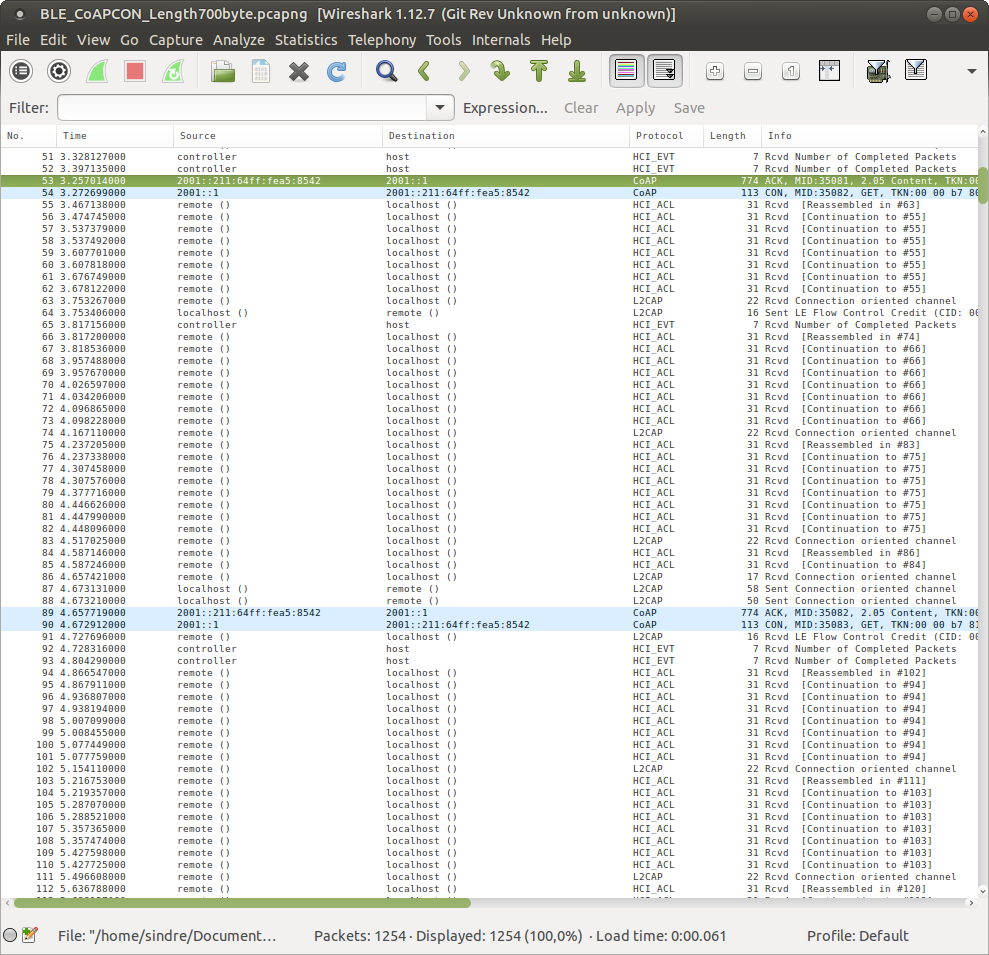
\includegraphics[width=\textwidth]{Wireshark700bytes2.png}    
%    \caption{Wireshark capture, CoAP CON, 700 bytes goodput}
%   \label{fig:coapCON700Wireshark}
%\end{figure}

\subsection{CoAP NON comparison}

A \gls{coap} \gls{non} request does not require a response in form of an \gls{ack}. This means that the 108 bytes sent to and handled by the end node can be skipped, which means less computational power in the end node and network capacity to the node is needed. This solution makes sense to use in networks where the demand for all data is low, since packets can be lost without the use of \glspl{ack}. As explained in chapter \ref{chp:measurements2}.1.1, the transfer frequency is limited using \gls{non} in this system, due to unstable results in tests at the beginning of the set up. The transfer rate is therefore set to one per second for this protocol. 

\todo{4 LEDs image?}

\begin{table}[ht]
\centering
\caption{Wireshark CoAP NON 0 bytes}
\label{coapNON0table}
\begin{tabular}{lllll}
\hline
Number & Time    & Protocol & Length & Info                             \\ \hline
%\rowcolor{blue} 
90     & 23.0405 & HCI\_ACL & 31     & Rcvd {[}Reassembled in \#92{]}   \\
91     & 23.0411 & HCI\_ACL & 31     & Rcvd {[}Continuation to \#90{]}  \\
92     & 23.1107 & L2CAP    & 9      & Rcvd Connection oriented channel \\
93     & 23.1109 & CoAP     & 76     & NON, MID:14, 2.05 Content        \\ \hline
\end{tabular}
\end{table}


A basic example of the \gls{coap} \gls{non} connection is shown in table \ref{coapNON0table}. The entire Wireshark capture can be seen in Appendix \ref{chp:appendix}. This is directly comparable to table \ref{coapCON0table}, that shows a Wireshark capture of \gls{coap} \gls{con} packages. It is easy to see that a lot fewer packages needs to be sent using \gls{ble}, without the use of \glspl{ack}. The total amount of bytes sent is 31+31+9=71 bytes, meaning three \gls{ble} packages and one \gls{6lowpan} packet. This is less than half of what was needed using \gls{coap} \gls{con}, where the 108 \gls{ack} packages was needed in addition. The packets are still recognizable the same way as before, the first packet is labeled \textit{[Reassembled in \#40]}, the second \textit{[Continuation to \#38]} and the last \textit{Connection oriented channel}.

Fewer packages sent means less energy used, less network capacity needed and less computational power in the end node. Hopefully this will lead to a higher percentage of goodput compared to throughput as well. it would therefore be interesting to compare the rest of the measured values.

\begin{table}[]
\centering
\caption{Wireshark CoAP NON 100 bytes}
\label{coapNON100table}
\begin{tabular}{lllll}
\hline
Number & Time    & Protocol & Length & Info   							  \\ \hline                          
39     & 11.0363 & CoAP     & 177    & NON, MID:2, 2.05 Content         \\
40     & 11.9452 & HCI\_ACL & 31     & Rcvd {[}Reassembled in \#45{]}   \\
41     & 11.9465 & HCI\_ACL & 31     & Rcvd {[}Continuation to \#40{]}  \\
42     & 12.0154 & HCI\_ACL & 31     & Rcvd {[}Continuation to \#40{]}  \\
43     & 12.0168 & HCI\_ACL & 31     & Rcvd {[}Continuation to \#40{]}  \\
44     & 12.0857 & HCI\_ACL & 31     & Rcvd {[}Continuation to \#40{]}  \\
45     & 12.0858 & L2CAP    & 29     & Rcvd Connection oriented channel \\
46     & 12.0860 & CoAP     & 177    & NON, MID:3, 2.05 Content         \\ \hline
\end{tabular}
\end{table}

Table \ref{coapNON100table} shows the case where 100 bytes of data are sent using \gls{coap} \gls{non}. This is directly comparable to the test shown in table \ref{coapCON100table}, where the same amount of data is sent over \gls{con}. The overall structure is the same as before. Since it is only one packet noted \textit{Reassembled in \#n}, which marks the beginning of a new \gls{6lowpan} packet. The total amount sent must therefore be under 270 bytes, which makes sense. The \gls{non} packet size is here 177 bytes, compared to 173 bytes in \gls{con}, which represents one more header field of 4 bytes needed in \gls{non}. Overall a small difference in the packets containing data, but as expected a lot more packets needs to be sent in total in \gls{con}.


Using these measurements the following plot could be drawn. 

%\begin{figure}[ht]
%    \centering
%    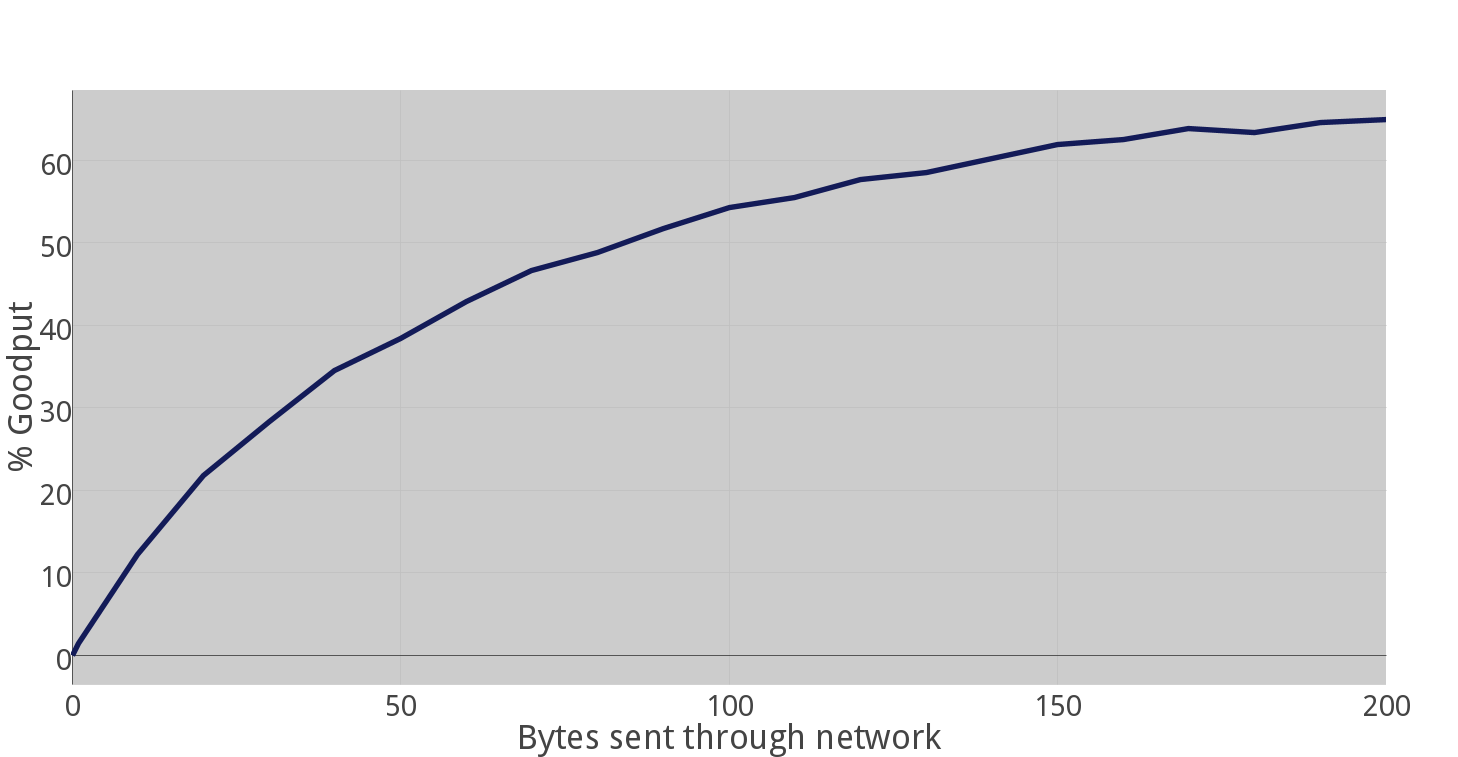
\includegraphics[scale=1.0]{NON0to200plotx09_thickerLineGRAY.png}    
%    \caption{NON 0-200 bytes }
%    \label{fig:NON0-200b}
%\end{figure}




\begin{figure}[ht]
    \centering
    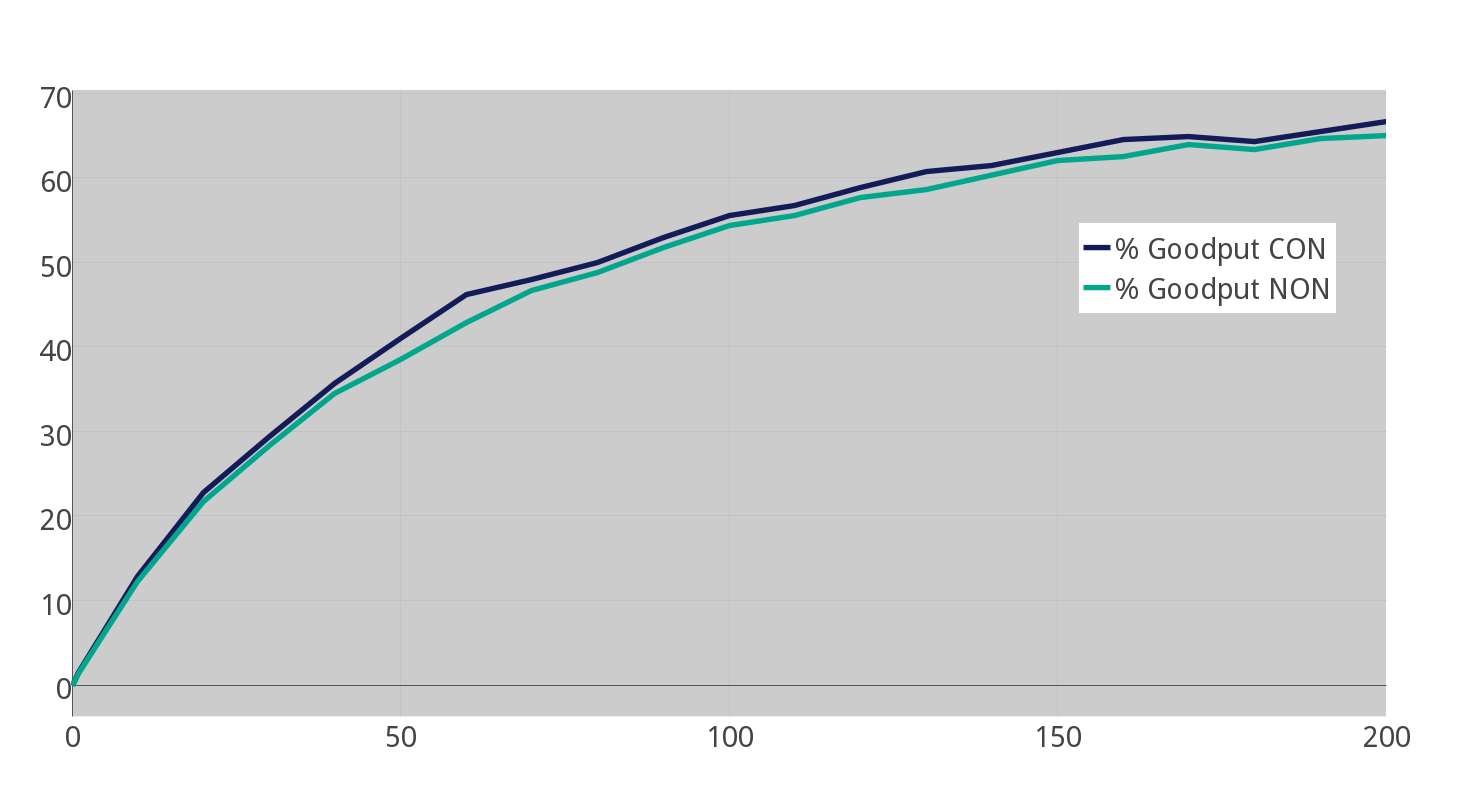
\includegraphics[scale=1.0]{CONvsNONplot_0-200_thickerGRAY.png}    
    \caption{CON vs NON 0-200 bytes}
    \label{fig:CONvsNON0-200}
\end{figure}

Figure \ref{fig:CONvsNON0-200} shows the comparison between sending between 0 and 200 bytes of useful data through the network at once. Keep in mind that this does not show sending rate per time (which will be discussed in chapter \todo{write chapter}), but percentage of the data sent that is useful data. \gls{con} can be sent much more often than \gls{non} in practice. It could therefore maybe be expected that this could give \gls{non} an advantage. \todo{<- Re-write}. \gls{non} does not need to send \glspl{ack} for every package, which should be an advantage concerning to maximize throughput. Still it is the more complex and more frequently sent \gls{con} that gets the best results in this test, with a small margin. 


\subsection{CoAP, testing with more data}

Table \ref{coapCON700table} shows a bigger and more complex case, where 700 bytes of data are being sent at once. In total 889 bytes are being sent, with a \gls{con} packet size of 774 bytes. This gives a percentage of goodput at 78.74 \%. The maximum packet length of a \gls{6lowpan} packet in this system of 270 bytes is therefore exceeded, as we can see in the figure. After 8 \gls{ble} packages of 31 bytes each has been sent, there is only room for 22 bytes in the last packet before the \gls{6lowpan} packet is full. This is repeated several times, once for each \gls{6lowpan} packet, until the last \gls{ble} packets at the size of 17 bytes. After this the standard packages for \gls{ack} and \textit{Number of completed packages} follows. This is in general a good example on how fragmentation of packets works in this system. 

\begin{table}[h]
\centering
\caption{Wireshark CoAP CON 700 bytes}
\label{coapCON700table}
\begin{tabular}{lllll}
\hline
Number & Time    & Protocol & Length & Info                             \\ \hline
%\rowcolor{blue} 
53     & 3.2570  & CoAP     & 774    & ACK, MID:35081, 2.05 Content     \\
%\rowcolor{38FFF8} 
54     & 3.2727  & CoAP     & 113    & CON, MID:35082, GET	              \\
55     & 3.4671  & HCI\_ACL & 31     & Rcvd {[}Reassembled in \#63{]}   \\
56     & 3.4747  & HCI\_ACL & 31     & Rcvd {[}Continuation to \#55{]}  \\
57     & 3.5374  & HCI\_ACL & 31     & Rcvd {[}Continuation to \#55{]}  \\
58     & 3.5375  & HCI\_ACL & 31     & Rcvd {[}Continuation to \#55{]}  \\
59     & 3.6077  & HCI\_ACL & 31     & Rcvd {[}Continuation to \#55{]}  \\
60     & 3.6078  & HCI\_ACL & 31     & Rcvd {[}Continuation to \#55{]}  \\
61     & 3.6767  & HCI\_ACL & 31     & Rcvd {[}Continuation to \#55{]}  \\
62     & 3.6782  & HCI\_ACL & 31     & Rcvd {[}Continuation to \#55{]}  \\
63     & 3.7533  & L2CAP    & 22     & Rcvd Connection oriented channel \\
64     & 3.7534  & L2CAP    & 16     & Sent LE Flow Control             \\
65     & 3.8172  & HCI\_EVT & 7      & Rcvd Number of Completed Packets \\
66     & 3.8172  & HCI\_ACL & 31     & Rcvd {[}Reassembled in \#74{]}   \\
67     & 3.8185  & HCI\_ACL & 31     & Rcvd {[}Continuation to \#66{]}  \\
68     & 3.9575  & HCI\_ACL & 31     & Rcvd {[}Continuation to \#66{]}  \\
69     & 3.9577  & HCI\_ACL & 31     & Rcvd {[}Continuation to \#66{]}  \\
70     & 4.0266  & HCI\_ACL & 31     & Rcvd {[}Continuation to \#66{]}  \\
71     & 4.0342  & HCI\_ACL & 31     & Rcvd {[}Continuation to \#66{]}  \\
72     & 4.0979  & HCI\_ACL & 31     & Rcvd {[}Continuation to \#66{]}  \\
73     & 4.0982  & HCI\_ACL & 31     & Rcvd {[}Continuation to \#66{]}  \\
74     & 4.1671  & L2CAP    & 22     & Rcvd Connection oriented channel \\
75     & 4.2372  & HCI\_ACL & 31     & Rcvd {[}Reassembled in \#83{]}   \\
76     & 4.2373  & HCI\_ACL & 31     & Rcvd {[}Continuation to \#75{]}  \\
77     & 4.3075  & HCI\_ACL & 31     & Rcvd {[}Continuation to \#75{]}  \\
78     & 4.3076  & HCI\_ACL & 31     & Rcvd {[}Continuation to \#75{]}  \\
79     & 4.3777  & HCI\_ACL & 31     & Rcvd {[}Continuation to \#75{]}  \\
80     & 4.4466  & HCI\_ACL & 31     & Rcvd {[}Continuation to \#75{]}  \\
81     & 4.4480  & HCI\_ACL & 31     & Rcvd {[}Continuation to \#75{]}  \\
82     & 4.4481  & HCI\_ACL & 31     & Rcvd {[}Continuation to \#75{]}  \\
83     & 4.5170  & L2CAP    & 22     & Rcvd Connection oriented channel \\
84     & 4.5871  & HCI\_ACK & 31     & Rcvd {[}Reassembled in \#86{]}   \\
85     & 4.5875  & HCI\_ACL & 31     & Rcvd {[}Continuation to \#84{]}  \\
86     & 4.6574  & L2CAP    & 17     & Rcvd Connection oriented channel \\
87     & 4.6731  & L2CAP    & 58     & Rcvd Connection oriented channel \\
88     & 4.6732  & L2CAP    & 50     & Rcvd Connection oriented channel \\
%\rowcolor[HTML]{38FFF8} 
89     & 4.6577  & CoAP     & 774    & ACK, MID:35082, 2.05 Content     \\
%\rowcolor[HTML]{38FFF8} 
90     & 4.6729  & CoAP     & 113    & NON, MID:35083, GET              \\ \hline
\end{tabular}
\end{table}


\newpage

\begin{figure}[ht]
    \centering
    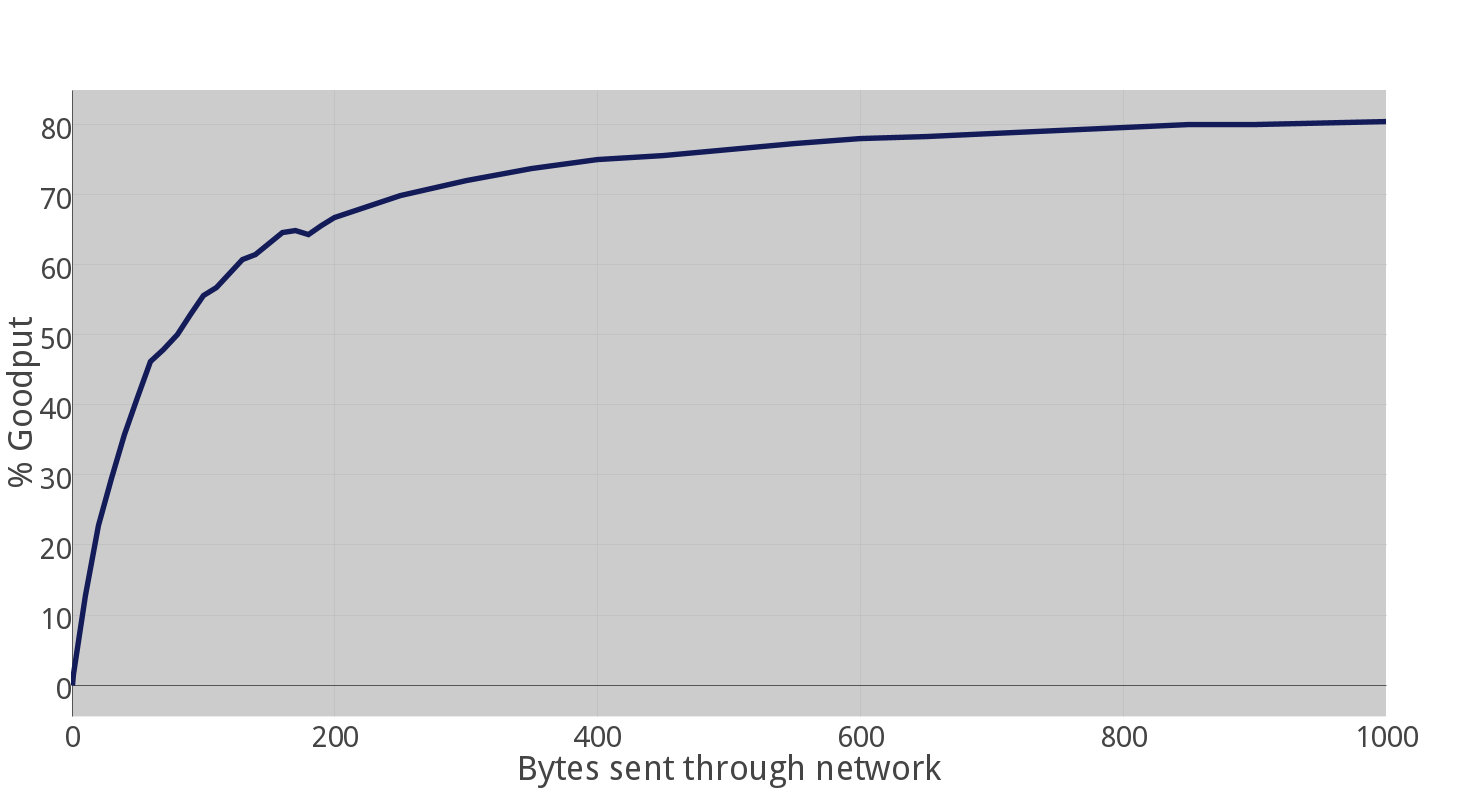
\includegraphics[width=\textwidth]{CON0toK_thickerGRAY.png}    
    \caption{CoAP CON plot, 200 bytes to 1 kB}
    \label{fig:plotCoAPCON200toK}
\end{figure}

Using these results it was possible to plot the graph in figure \ref{fig:plotCoAPCON200toK} \todo{Make graph more clear}. Here it is easy to see the same trends as in  \ref{fig:coapCON0200}, but in more detail over a wider span of bytes sent. These results are as expected after the previous tests, and in compliance with the calculations done in equation 4.1. 

In this example points in the graph was denoted every 50th byte sent. This gives us \todo{set in graph for 0-1000 before this, to see the flatness?}


%\begin{figure}[ht]
%    \centering
%    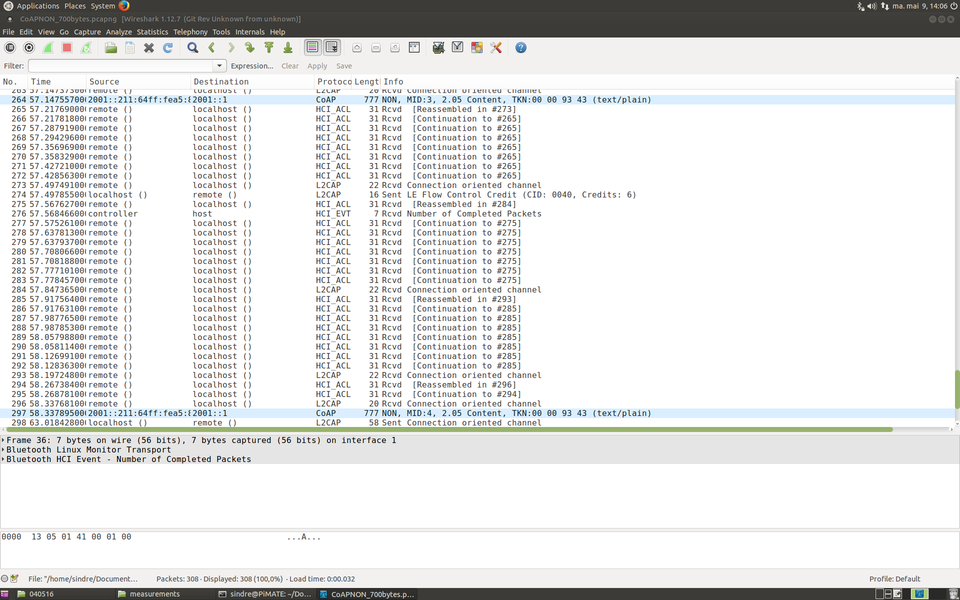
\includegraphics[scale=0.40]{rsz_1coapnon_wireshark700fullscreen.png}    
%    \caption{CoAP NON 700 bytes Wireshark capture}
%    \label{fig:NON7000bytesFullWireshark}
%\end{figure}

 


\begin{table}[ht]
\centering
\caption{Wireshark CoAP NON 700 bytes}
\label{coapNON700table}
\begin{tabular}{lllll}
\hline
Number & Time    & Protocol & Length & Info                             \\ \hline
264    & 57.1476 & CoAP     & 777    & NON, MID:3, 2.05 Content         \\
265    & 57.2177 & HCI\_ACL & 31     & Rcvd {[}Reassembled in \#273{]}  \\
266    & 57.2178 & HCI\_ACL & 31     & Rcvd {[}Continuation to \#265{]} \\
267    & 57.2879 & HCI\_ACL & 31     & Rcvd {[}Continuation to \#265{]} \\
268    & 57.2943 & HCI\_ACL & 31     & Rcvd {[}Continuation to \#265{]} \\
269    & 57.3570 & HCI\_ACL & 31     & Rcvd {[}Continuation to \#265{]} \\
270    & 57.3583 & HCI\_ACL & 31     & Rcvd {[}Continuation to \#265{]} \\
271    & 57.4272 & HCI\_ACL & 31     & Rcvd {[}Continuation to \#265{]} \\
272    & 57.4286 & HCI\_ACL & 31     & Rcvd {[}Continuation to \#265{]} \\
273    & 57.4975 & L2CAP    & 22     & Rcvd Connection oriented channel \\
274    & 57.4979 & L2CAP    & 16     & Sent LE Flow Control             \\
275    & 57.5676 & HCI\_ACL & 31     & Rcvd {[}Reassembled in \#284{]}  \\
276    & 57.5685 & HCI\_EVT & 7      & Rcvd Number of Completed Packets \\
277    & 57.5753 & HCI\_ACL & 31     & Rcvd {[}Continuation to \#275{]} \\
278    & 57.6378 & HCI\_ACL & 31     & Rcvd {[}Continuation to \#275{]} \\
279    & 57.6379 & HCI\_ACL & 31     & Rcvd {[}Continuation to \#275{]} \\
279    & 57.7080 & HCI\_ACL & 31     & Rcvd {[}Continuation to \#275{]} \\
280    & 57.7082 & HCI\_ACL & 31     & Rcvd {[}Continuation to \#275{]} \\
281    & 57.7771 & HCI\_ACL & 31     & Rcvd {[}Continuation to \#275{]} \\
282    & 57.7785 & HCI\_ACL & 31     & Rcvd {[}Continuation to \#275{]} \\
283    & 57.7785 & HCI\_ACL & 31     & Rcvd {[}Continuation to \#275{]} \\
284    & 57.8474 & L2CAP    & 22     & Rcvd Connection oriented channel \\
285    & 57.9176 & HCI\_ACL & 31     & Rcvd {[}Reassembled in \#293{]}  \\
286    & 57.9176 & HCI\_ACL & 31     & Rcvd {[}Continuation to \#285{]} \\
287    & 57.9878 & HCI\_ACL & 31     & Rcvd {[}Continuation to \#285{]} \\
288    & 57.9879 & HCI\_ACL & 31     & Rcvd {[}Continuation to \#285{]} \\
289    & 58.0580 & HCI\_ACL & 31     & Rcvd {[}Continuation to \#285{]} \\
290    & 58.0581 & HCI\_ACL & 31     & Rcvd {[}Continuation to \#285{]} \\
291    & 58.1270 & HCI\_ACL & 31     & Rcvd {[}Continuation to \#285{]} \\
292    & 58.1284 & HCI\_ACL & 31     & Rcvd {[}Continuation to \#285{]} \\
293    & 58.1972 & L2CAP    & 22     & Rcvd Connection oriented channel \\
294    & 58.2673 & HCI\_ACK & 31     & Rcvd {[}Reassembled in \#296{]}  \\
295    & 58.2688 & HCI\_ACL & 31     & Rcvd {[}Continuation to \#294{]} \\
296    & 58.3378 & L2CAP    & 20     & Rcvd Connection oriented channel \\
297    & 58.3379 & CoAP     & 777    & NON, MID:4, 2.05 Content         \\ \hline
\end{tabular}
\end{table}

\newpage

Table \ref{coapNON700table} shows the case where 700 bytes where sent at once through the network, using \gls{coap} \gls{non}. The \gls{non} packet size is at 777 bytes, which is as expected from the previous tests. This means 4 bytes larger than the same test using \gls{con}, meaning an additional header field. 

\begin{equation} \label{lessThanHAlfAPercentCalculation}
    \frac{78,47}{78,74} \approx 0,9966  \rightarrow 100 \% - 99,66 \% = 0,34 \%
\end{equation}


Calculations in equation \ref{lessThanHAlfAPercentCalculation} show that the goodput here is 78,47 \%, compared to 78,74 \% in \gls{con}. The difference between these two is \textit{0,34 \%}, which in this case is considered \textit{very} small. This can also be seen clearly in \ref{fig:CONvsNON0-1000}. Because of this, it was concluded that the results for using \gls{non} and \gls{con} can be considered as negligible for transmissions larger than 1 kB. Tests with larger amounts of data than this at once was therefore not conducted in this project.  



\begin{figure}[ht]
    \centering
    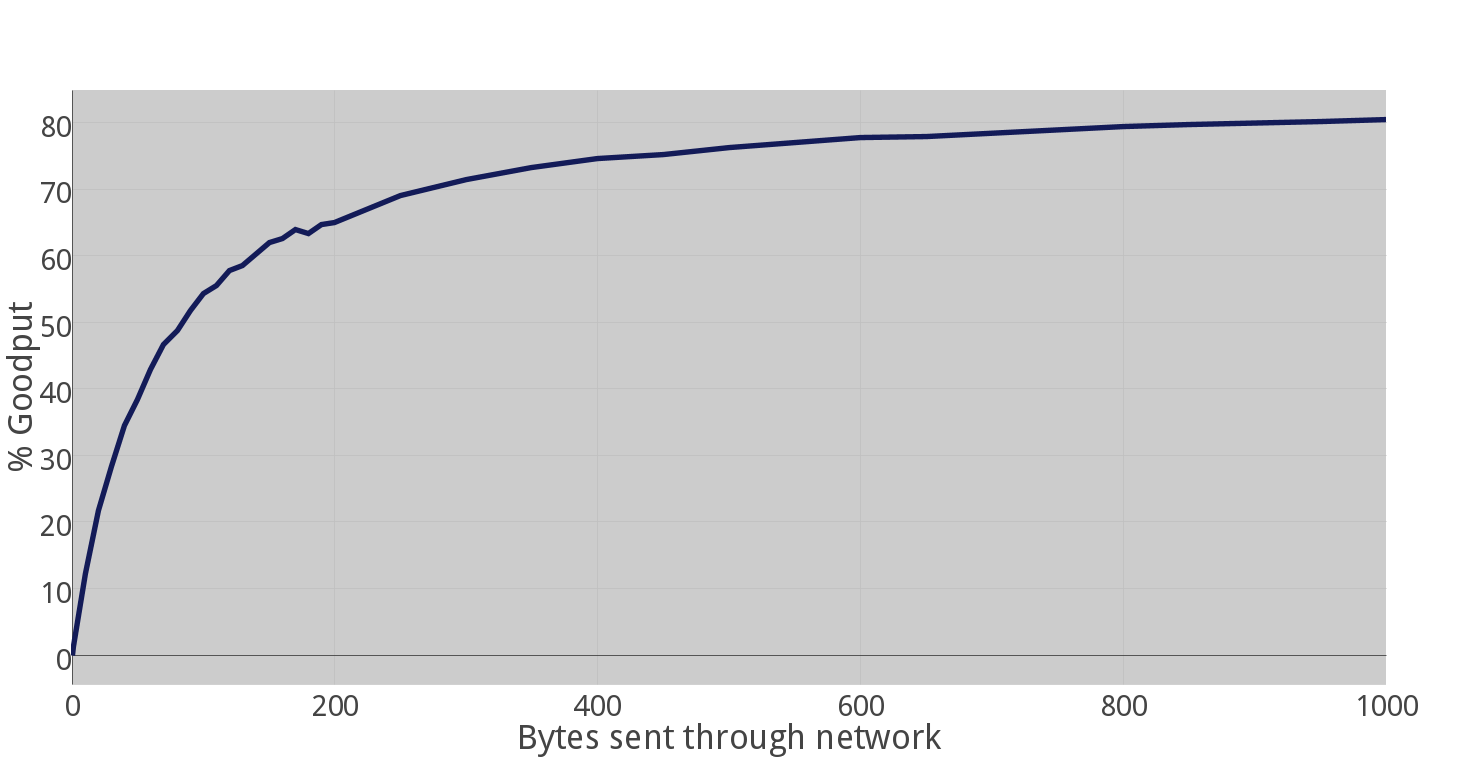
\includegraphics[scale=1.0]{NON_0toKplotx09_thickerLineGRAY.png}    
    \caption{NON 0-1000 bytes}
    \label{fig:NON0-kb}
\end{figure}

The entire scope of the tests done on \gls{coap} \gls{non} in this system is shown in figure \ref{fig:NON0-kb}. Given these results, it can be concluded that to send less data than 200 bytes at the time is not preferable, since the percentage of goodput compared to the total amount sent can be very low. On the other hand, the graph stabilizes around 75-80 \%. Given these measurements it looks like 400 bytes and bigger packets are preferable in this system. The system shows no signs of weakness as the packet size grows, and it will therefore be possible to send as large packets as needed until the limitations of \gls{ble} with the same amount of goodput at about 80 \%. 

\todo{Remove figure 4.8 200-1000?}
\begin{figure}[ht]
    \centering
    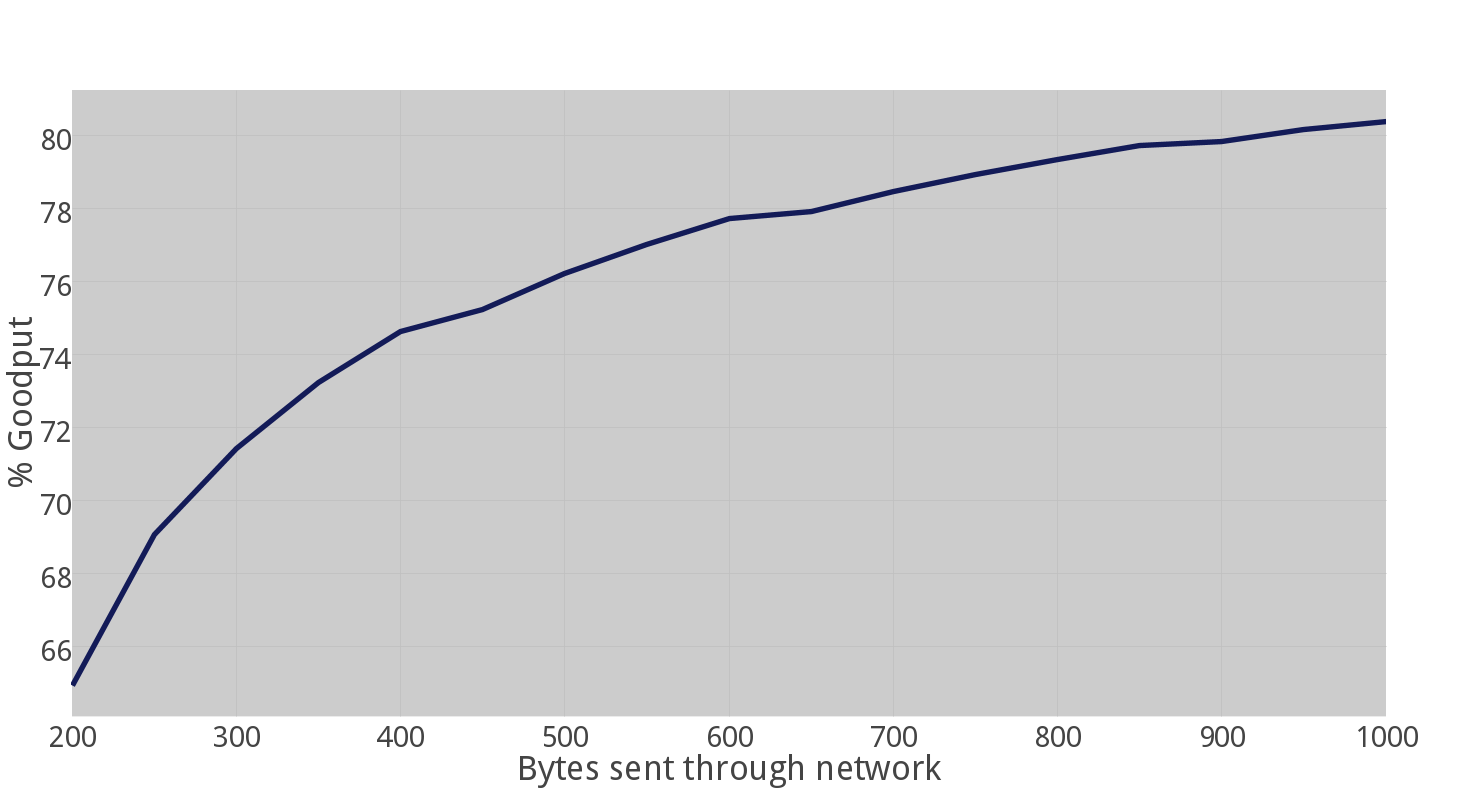
\includegraphics[scale=1.0]{NON_200toKplotx09_thickerLineGRAY.png}    
    \caption{NON 200-1000 bytes}
    \label{fig:NON200-kb}
\end{figure}



%\begin{figure}[ht]
%    \centering
%    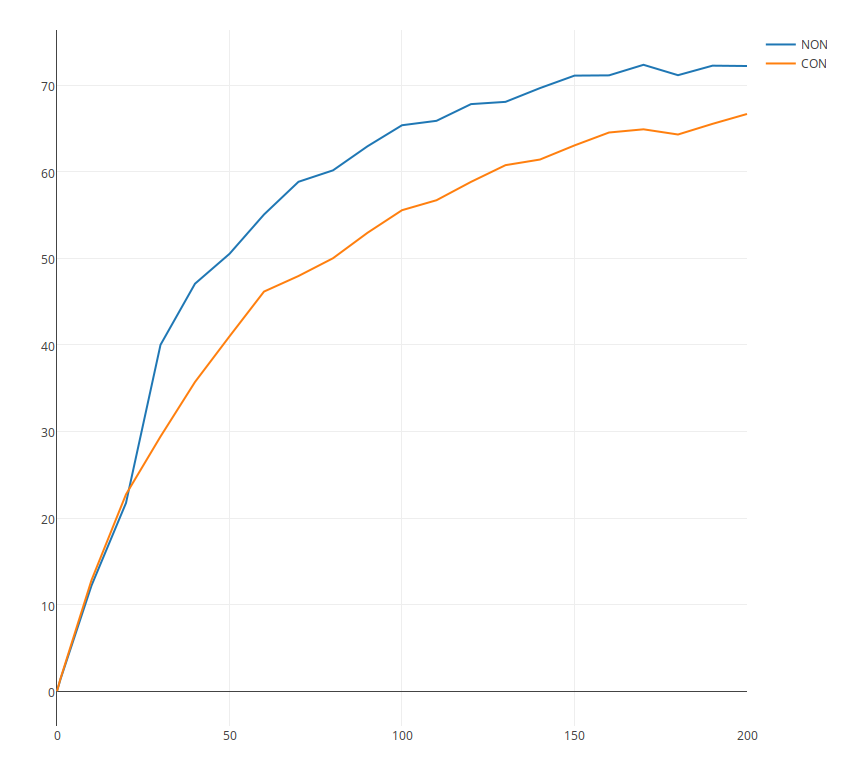
\includegraphics[scale=0.45]{CONvsNON1.png}    
%    \caption{CON vs NON}
%    \label{fig:CONvsNON}
%\end{figure}





%\begin{figure}[ht]
%    \centering
%    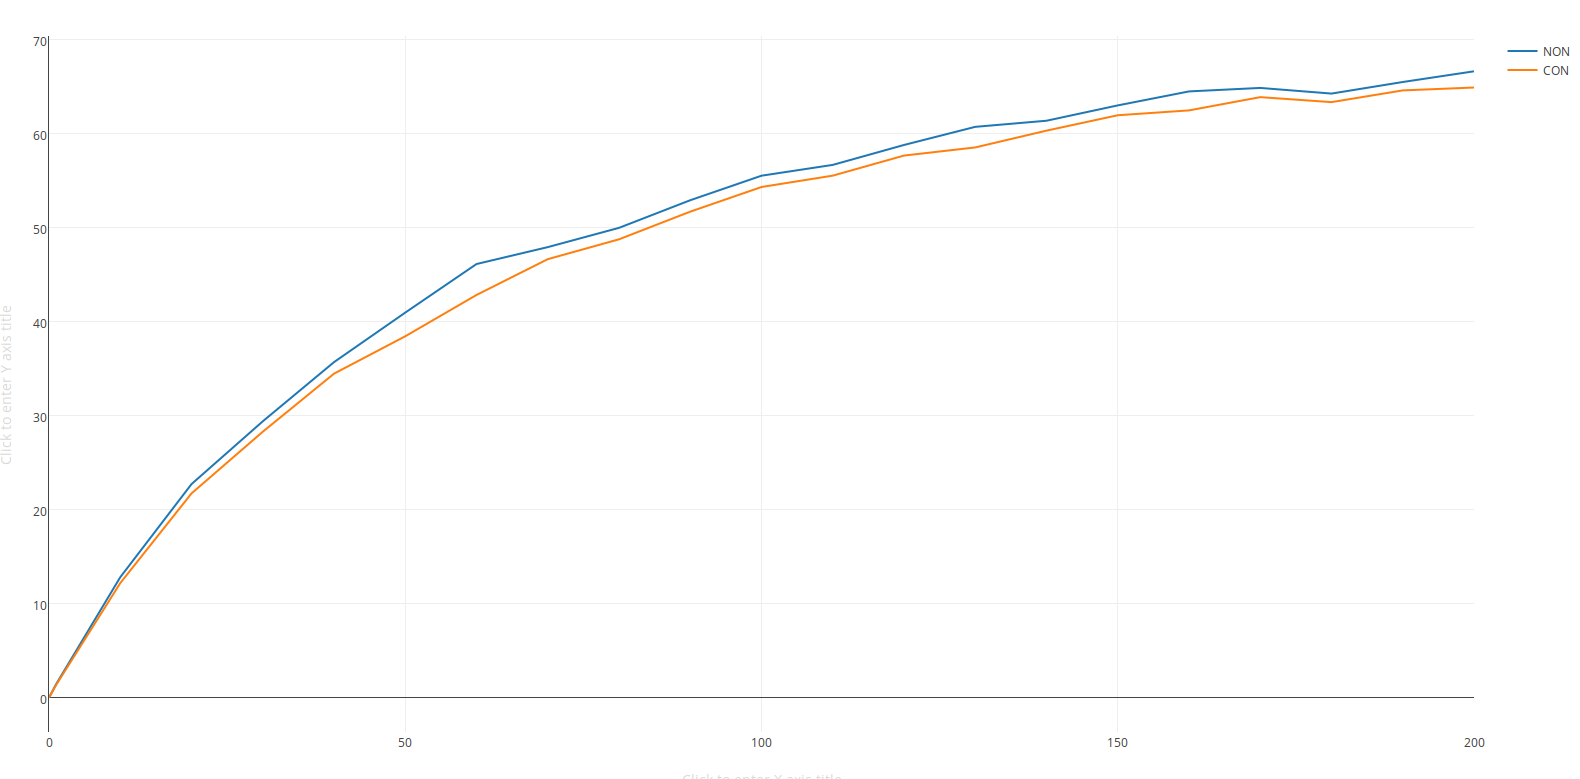
\includegraphics[scale=0.25]{CONvsNON0-200_2.png}    
%    \caption{CON vs NON 0-200 bytes number 2}
%    \label{fig:CONvsNON0-200}
%\end{figure}




\subsection{Discussion}

\section{Comparison}



\begin{figure}[ht]
    \centering
    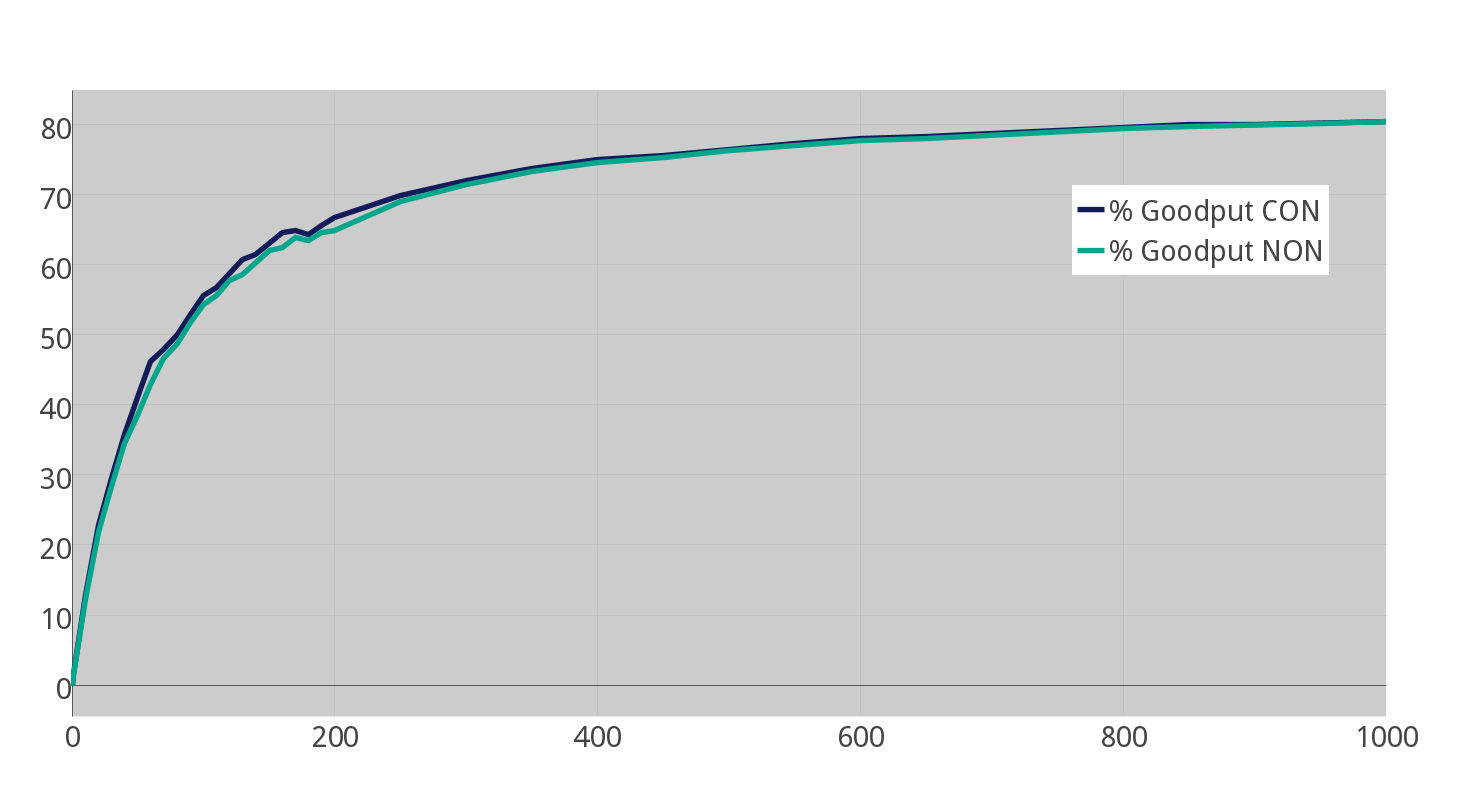
\includegraphics[scale=1.0]{CONvsNONplot_0-k_thickerGRAY.png}    
    \caption{CON vs NON 0-1000 bytes}
    \label{fig:CONvsNON0-1000}
\end{figure}

\begin{figure}[ht]
    \centering
    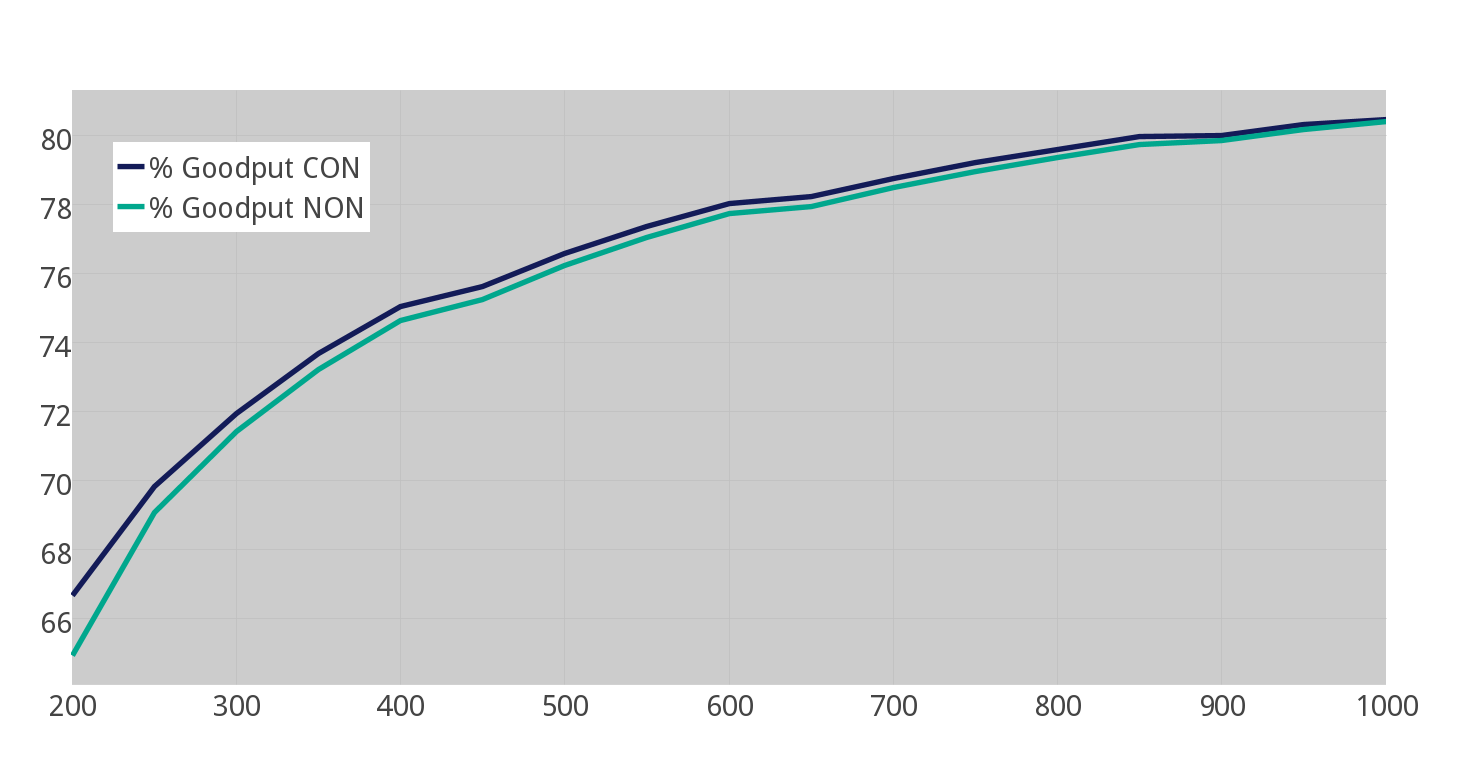
\includegraphics[scale=1.0]{CONvsNONplot_200-k_thickerGRAY.png}    
    \caption{CON vs NON 200-1000 bytes}
    \label{fig:CONvsNON200-1000}
\end{figure}

\subsection{Goodput per time interval}

Previous sections in this chapter has shown the percentage of bytes sent through that has been goodput, useful data, compared to the total amount of bytes. This is a good overview of how the protocols are able to exploit the network, and tells a lot about the different protocols. In a real world scenario however, the actual \textit{throughput per time} would be more relevant, since this tells how much data can be transported for every second.

\gls{coap} \gls{con} and \gls{non} has been compared in this thesis, but in the system build \gls{non} was quite unstable at high transfer rates, as explained in chapter \ref{chp:architecture}.1. Because of this, \gls{con} seems like a better solution only considering the number of bytes transferred per second. As it turns out, this depends. 

As seen in Table \todo{insert table}, this might be a too early conclusion.

The table shows timestamps of packets received on the Raspberry Pi, sent with both \gls{con} and \gls{non}. Packets was captured with Wireshark, and the timestamp is created by Wireshark on the form \textit{number of seconds since start of capture}. The first value for each packet size in the table therefore approximately notes the number of seconds from the connection starts until the first packet containing useful data has arrived \footnote{values far off from the expected results due to e.g. connection issues have been excluded in calculations }. The first thing that is noticeable here is the big difference before useful data can be received. Equation \ref{averageStartTimeCON} shows the calculations of average start time on \gls{con}, which is a lot higher than for \gls{non} shown in equation \ref{averageStartTimeNON}. The main reason for this is that the \gls{non} needs to have a connection establishment using \gls{con} packets with \glspl{ack} without data before \gls{non} packets can be transferred. In addition severe connection issues was experienced in a much higher grade using \gls{non} than \gls{con}, especially for packets larger than 500 bytes, as shown in table \todo{Refer to table}.  

\todo{DROP THESE} 

\begin{equation} \label{averageStartTimeCON}
     \frac{3.4677+2.2425+4.0885+5.2941+3.3297+1.3398+4.6184+3.257+3.4062}{9} \approx 3
\end{equation}


\begin{equation} \label{averageStartTimeNON}
	\frac{10.1609+10.0567+9.4627+8.5798+28.3489+29.069}{6} \approx 16
\end{equation}

These two equations 


Figure \todo{Tegn graf om hvor mange pakker som kan sendes per sekund} 

\todo{Tegn graf om hvor lang tid det tar aa sende x andtall pakker, feks 13 eller 15?}

There are in general two ways to measure throughput compared to time, the number of seconds it takes to transfer a known number of bytes, and the number of bytes that are transported on average every second. 





%\section{BLE}


\section{Time spent in network}

The previous tests shows 



Calcumate time for \gls{coap} \gls{non}, 700 bytes sent:

\begin{equation}
    ((55.9578-54.7750)+(57.1476-55.9578)+(58.3379-57.1476))/3 = 1.1876
\end{equation}

 	0.1876/3 = 0.0625


\section{Quantity test}

This section will show a test of several nRF52 devices connected to the same Pi at the same time, to ensure stability and performance in the network. Even though this puts more pressure on both the network and the Pi, it is not expected to be considerably noticed in the transportation of packets. 


\todo{Do measurements of several nRF52s. Write new python script to gather data from all of these. Add this to the Appendix}

